\chapter[Asian options and control variates]{Asian options\\ and control variates}
\label{cap:asiatiche}

The arithmetic Asian option is the textbook case in which Monte Carlo is unavoidable but can be made very efficient.
Its geometric ``twin'' has a closed-form formula, and that formula is used twice: as an oracle for the Monte Carlo and
as a control variate. In this chapter we derive the formula, the optimal control coefficient and the variance-reduction
factor, then we see why the control is valid only under Black and which error surfaced under Heston.

\section{The product}
An arithmetic Asian option pays on the \emph{average} of the prices observed on $n$ fixed dates (\emph{fixings})
$t_1<\dots<t_n$ in $[0,T]$:
\begin{equation}
A=\frac1n\sum_{i=1}^nS_{t_i},\qquad\text{payoff }(\theta(A-K))^+\ \text{paid at }T .
\end{equation}
Why they exist: they are cheaper than vanillas (the average fluctuates less than a single price) and they are robust
to a single anomalous or manipulated settlement price. The geometric twin uses $G=\big(\prod_iS_{t_i}\big)^{1/n}$. On
the same paths we denote the discounted payoffs by
\[
Y=\DF\,(\theta(A-K))^+,\qquad X=\DF\,(\theta(G-K))^+.
\]

\section{The fixing forwards}
With deterministic rates and carry, the expected value of each fixing is the forward for that date:
\begin{equation}\label{eq:forward-fixing}
\E[S_{t_i}]=F(0,t_i)=:F_i,\qquad\E[A]=\bar A_F=\frac1n\sum_iF_i,\qquad V_A=\DF\cdot\E[(\theta(A-K))^+].
\end{equation}
\emph{Why.} $S_t=F(t,T)\,F(0,t)/F(0,T)$ and $F(\cdot,T)$ is a martingale, hence $\E S_t=F(0,t)$. With a constant
carry $b$, $F_i=F\,e^{-b(T-t_i)}$ and $\partial F_i/\partial b=-(T-t_i)F_i$: the price is sensitive to the timing of
dividends.
\begin{attenzione}
The price depends on the \emph{whole} curve $F_1,\dots,F_n$, not only on $F(0,T)$. The Monte Carlo and the closed
form use the same curve, so a Monte Carlo versus formula comparison \emph{cannot} reveal a wrong curve (for example
$F(0,T)$ for every fixing, or interpolating $F$ instead of $\ln F$). The curve builder must be tested separately. In
the project, for the SPX, $\ln F$ (and $\ln\DF$) is interpolated linearly between the expiries obtained from parity;
a fixing at time zero enters with $F(0,0)=S_0$, supplied by the caller.
\end{attenzione}

\section{The closed form for the geometric (discrete Kemna--Vorst)}
Under Black every $S_{t_i}$ is lognormal, but a \textbf{sum} of lognormals is not lognormal: there is no closed form
for $A$. A \textbf{product} of lognormals, on the other hand, is lognormal, because the logarithm turns the product
into a sum of Gaussians. We derive the formula for arbitrary dates.

\noindent\textbf{Step 1 (law of the fixings).} Let $V(t)=\int_0^t\sigma^2(s)\dd s$ be the total variance up to $t$
(with constant $\sigma$, $V(t)=\sigma^2t$). As in Chapter~\ref{cap:strumenti},
\[
\ln S_{t_i}=\ln F_i-\tfrac12V(t_i)+M_{t_i},\qquad M_t=\int_0^t\sigma\dd W,\qquad\Cov(M_s,M_t)=V(\min(s,t)).
\]
The covariance of a stochastic integral is the variance accumulated up to the smaller time.

\noindent\textbf{Step 2 (mean of $\ln G$).} $\ln G=\frac1n\sum_i\ln S_{t_i}$ is a linear combination of Gaussians,
hence Gaussian. Its mean is
\begin{equation}\label{eq:mu-G}
\mu_G=\ln\bar G_F-\tfrac12\bar V,\qquad\bar G_F=\Big(\prod_iF_i\Big)^{1/n},\qquad\bar V=\frac1n\sum_iV(t_i).
\end{equation}

\noindent\textbf{Step 3 (variance of $\ln G$).} It is the variance of $\frac1n\sum_iM_{t_i}$:
\begin{equation}\label{eq:sigma-G}
\sigma_G^2=\frac1{n^2}\sum_{i,j}V(\min(t_i,t_j))=\frac1{n^2}\sum_{i=1}^n(2n-2i+1)\,V(t_i)=\sum_{k=1}^nw_k^2\,\Delta V_k ,
\end{equation}
with $\Delta V_k=V(t_k)-V(t_{k-1})$, $t_0=0$ and $w_k=(n-k+1)/n$. The second form counts the pairs $(i,j)$ whose
minimum equals $i$: there are $2(n-i)+1$ of them. The third (Abel form) writes $\sum_iM_{t_i}=\sum_k(n-k+1)\Delta M_k$
with independent increments: each increment is shared by all later fixings, and therefore carries weight
$\big((n-k+1)/n\big)^2$.

\noindent\textbf{Step 4 (forward of $G$).} For a lognormal $\E G=e^{\mu_G+\sigma_G^2/2}$:
\begin{equation}\label{eq:FG}
F_G=\bar G_F\exp\!\big(-\tfrac12(\bar V-\sigma_G^2)\big).
\end{equation}

\noindent\textbf{Step 5 (Black formula).} The derivation of Chapter~\ref{cap:black} uses only the fact that
$\ln F_T\sim\N(\ln F-s^2/2,\,s^2)$. Here $\ln G\sim\N(\ln F_G-\sigma_G^2/2,\,\sigma_G^2)$, hence
\begin{equation}\label{eq:kv}
V_G=\DF\,\theta\big[F_G\,\Phi(\theta d_1)-K\,\Phi(\theta d_2)\big],\qquad
d_{1,2}=\frac{\ln(F_G/K)}{\sigma_G}\pm\frac{\sigma_G}2 .
\end{equation}
It is Black with forward $F_G$ and total volatility $\sigma_G$ in place of $\sigma\sqrt T$.

\begin{idea}[title={Two facts to remember}]
\begin{itemize}
\item \textbf{Convexity.} The factor $e^{-\frac12(\bar V-\sigma_G^2)}\le1$ says that the forward of $G$ is \emph{not}
the geometric mean of the forwards. The variance of an average does not exceed the average of the variances
($\sigma_G^2\le\bar V$), and by AM--GM $\bar G_F\le\bar A_F$; hence $F_G\le\bar G_F\le\bar A_F$.
\item \textbf{Reduced volatility.} With equally spaced fixings $t_i=iT/n$ ($t_0$ excluded) and constant $\sigma$, from
$\sum i=n(n+1)/2$ and $\sum(2n-2i+1)\,i=n(n+1)(2n+1)/6$:
\[
\sigma_G^2=\sigma^2T\,\frac{(n+1)(2n+1)}{6n^2}\ \xrightarrow{\ n\to\infty\ }\ \frac{\sigma^2T}{3}.
\]
For a continuous average the effective volatility is $\sigma/\sqrt3\approx0.58\,\sigma$: this is why Asians are
cheaper than vanillas.
\end{itemize}
\end{idea}

\begin{attenzione}[title={\texorpdfstring{Conventions: the fixing at $t=0$ and the continuous formula}{Conventions: the
fixing at t=0 and the continuous formula}}]
In the literature some authors include today's fixing ($n+1$ fixings $t_k=kT/n$, $k=0,\dots,n$, divisor $n+1$), others
do not. With the fixing at zero $\sigma_G^2=\sigma^2T\,(2n+1)/(6(n+1))$: the volatility is smaller by exactly the factor
$n/(n+1)$, that is by 7.7\% at $n=12$ (put the other way round, the convention without the fixing at zero gives a
volatility 8.3\% larger). Published values cannot be reproduced with the wrong convention: this is why the product
stores the vector of dates explicitly. Using the continuous formula for discrete fixings is another error: at $n=12$
(fixing at zero included) the continuous formula gives 4.791541 against 4.703634 at $K=100$, that is 0.0879 more.
\end{attenzione}

\begin{esempio}[title={Example: Fusai--Meucci (2008)}]
$S_0=100$, $r=3.67\%$, $\sigma=17.801\%$, $T=1$, fixings $t_k=k/n$ with the fixing at zero. In forward form
$F_k=100e^{0.0367t_k}$ and $\DF=e^{-0.0367}$. Published values for the geometric Asian:
\begin{center}
\small
\begin{tabular}{llll}
\toprule
& $K=90$ & $K=100$ & $K=110$\\
\midrule
$n=12$ & 11.66744 & 4.703634 & 1.251243\\
$n=50$ & 11.7076\phantom{0} & 4.769273 & 1.299134\\
$n=250$ & 11.71856 & 4.787024 & 1.312165\\
continuous & 11.72135 & 4.791541 & 1.315486\\
\bottomrule
\end{tabular}
\end{center}
Formula \eqref{eq:kv} reproduces them within $1.28\times10^{-4}$ (tolerance $3\times10^{-4}$). The gap is not an
error: the printed $\sigma$ is rounded, and a single unrounded value, $\sigma=0.1780163$, reproduces all 12 values
within $3.6\times10^{-6}$.
\end{esempio}

\section{The geometric control variate}
\subsection{The idea}
I want to estimate $\E Y$ (the discounted arithmetic payoff). On the same paths I have another variable $X$ (the
geometric payoff) whose mean $\mu_X=V_G$ I know \emph{exactly}. Then, for any $c$,
\begin{equation}\label{eq:cv}
\hat V_{CV}=\frac1N\sum_{i=1}^N\big[Y_i-c\,(X_i-\mu_X)\big]
\end{equation}
has the same mean as $\bar Y$ (the added term has zero mean), but can have a much smaller variance.

\subsection{The optimal coefficient and the reduction factor}
\noindent\textbf{Step 1.} $\Var(Y-cX)=\Var Y-2c\Cov(X,Y)+c^2\Var X$ is a parabola in $c$.

\noindent\textbf{Step 2.} Differentiating and setting to zero: $c^*=\Cov(X,Y)/\Var X$.

\noindent\textbf{Step 3.} Substituting, with $\rho_{XY}=\Cov(X,Y)/\sqrt{\Var X\Var Y}$:
\begin{equation}\label{eq:vr}
\Var(Y-c^*X)=\Var Y\,\big(1-\rho_{XY}^2\big),\qquad
\boxed{\mathrm{VR}=\frac{\Var Y}{\Var(Y-c^*X)}=\frac{1}{1-\rho_{XY}^2}}
\end{equation}
VR is the variance-reduction factor: with the same number of paths the standard error is divided by
$\sqrt{\mathrm{VR}}$. Correlations 0.9, 0.99, 0.999 give VR $=5.3$, 50, 500. The cost is negligible: $G$ is computed on
the same paths with one extra sum of logarithms.

\paragraph{Estimating $c$.} In practice $\hat c$ is the slope of the (OLS) regression of $Y$ on $X$ on the same
paths. This introduces a bias $-\Cov(\hat c,\bar X)=O(1/N)$, negligible compared with the standard error
$O(N^{-1/2})$. If exact unbiasedness is required, one uses $c=1$ or estimates $\hat c$ on a separate pilot sample. With
$\hat c$ from OLS and the same degrees of freedom, the estimated factor $s_Y^2/s_e^2$ coincides with
$1/(1-\hat\rho^2)$ (in the project, to $10^{-10}$).

\begin{perche}[title={Why arithmetic and geometric are so highly correlated}]
With $y_i=\ln S_{t_i}$ and $\bar y$ their mean,
\[
\frac AG=\frac1n\sum_ie^{y_i-\bar y}=1+\frac1{2n}\sum_i(y_i-\bar y)^2+\dots
\]
because the linear term sums to zero. Hence $A-G$ is \emph{second order} in the dispersion of the fixings,
$O(\sigma^2T)\cdot F$, while the payoffs vary at first order, $O(\sigma\sqrt T)\cdot F$. Near the money and with
moderate $\sigma\sqrt T$ the two payoffs move almost one for one: $c^*\approx1$ and $\rho\to1$. A rule of thumb also
follows: $1-\rho^2$ scales as the square of the ratio between the two orders, that is as $\sigma^2T$, and therefore
$\mathrm{VR}\sim1/\sigma^2$. Far from the money, instead, both payoffs are almost always zero, the exercise sets
$\{A>K\}\supseteq\{G>K\}$ differ in relative terms, and the correlation drops.
\end{perche}

\subsection{The measured factors}
\begin{figure}[htbp]
\centering
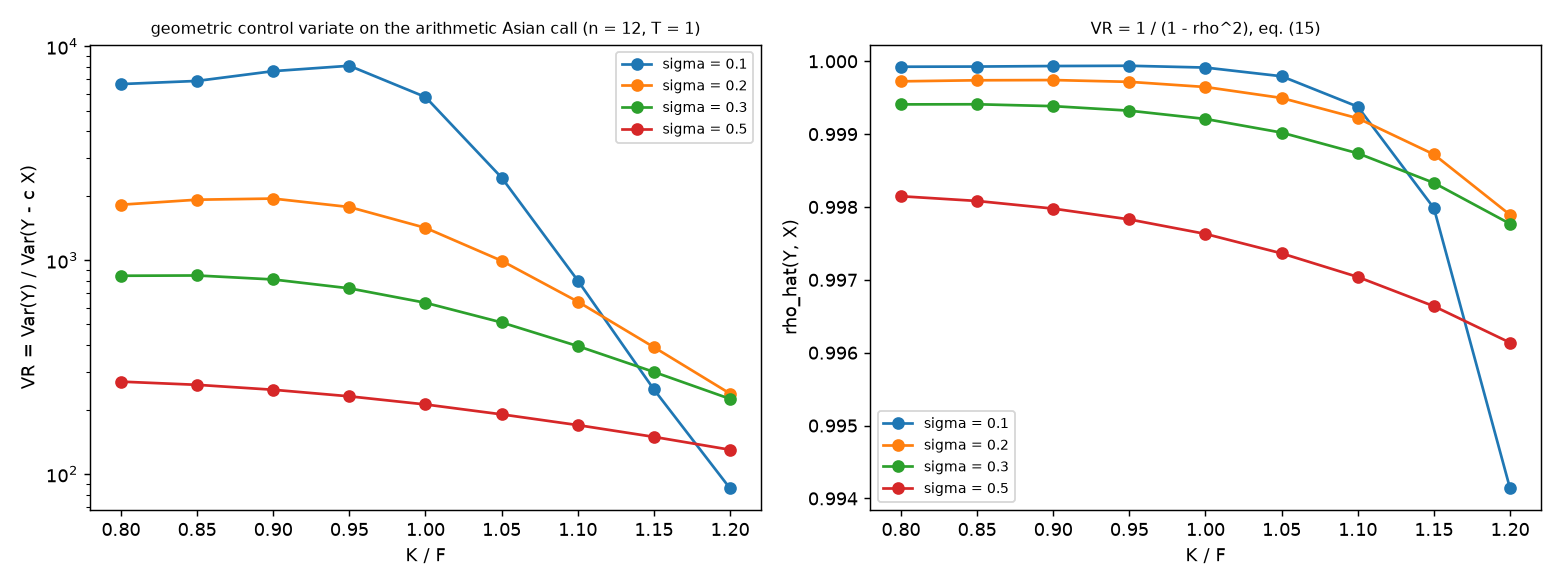
\includegraphics[width=\textwidth]{asian_cv_vr.png}
\caption{Arithmetic Asian call, $n=12$, $T=1$, $2\times10^5$ paths per $\sigma$. Left: the variance-reduction factor
$\mathrm{VR}=\Var(Y)/\Var(Y-\hat cX)$ on a log scale, against $K/F$; right: the estimated correlation
$\hat\rho(Y,X)$.}
\label{fig:asian-cv-vr}
\end{figure}

Figure~\ref{fig:asian-cv-vr} shows VR and $\hat\rho$ for four volatilities; Table~\ref{tab:asian-vr} reports the
at-the-money values ($K/F=1$).
\begin{table}[htbp]
\centering
\small
\caption{Control variate at the money ($K/F=1$, $n=12$, $T=1$, $2\times10^5$ paths).}
\label{tab:asian-vr}
\begin{tabular}{lcccc}
\toprule
$\sigma$ & 0.1 & 0.2 & 0.3 & 0.5\\
\midrule
VR & 5793 & 1416 & 632 & 211\\
$\hat\rho$ & 0.99991 & 0.99965 & 0.99921 & 0.99763\\
$\hat c$ & 1.014 & 1.030 & 1.047 & 1.086\\
\bottomrule
\end{tabular}
\end{table}

The ratios between successive VRs are 4.1, 2.2 and 3.0, against the squared ratios of $\sigma$, 4, 2.25 and 2.8: the
rule $\mathrm{VR}\sim1/\sigma^2$ works well at the money. Away from the money VR collapses, and faster when $\sigma$ is
small: at $\sigma=0.1$ it goes from a maximum of 8113 ($K/F=0.95$) to 85.5 at $K/F=1.2$ ($\hat\rho=0.9941$,
$\hat c=1.12$). This is why one always states \emph{which} $\sigma$ and strike a VR refers to.

\begin{esempio}[title={\texorpdfstring{Example: Fusai--Meucci, arithmetic with $n=12$}{Example: Fusai--Meucci,
arithmetic with n=12}}]
With $2\times10^5$ paths: at $K=100$ the control-variate price is 4.88132 with SE $3.8\times10^{-4}$, against the
published value 4.88210. Plain Monte Carlo on the same paths would have SE $1.5\times10^{-2}$. VR $=1924$, 1608 and 612
at $K=90$, 100, 110 ($\hat\rho=0.99974$, 0.99969, 0.99918). All nine published values ($n=12$, 50, 250) are within
3 SE. A comparison between the control-variate price and plain Monte Carlo on \emph{independent} seeds ($\sigma=0.3$,
$n=12$) gives $\max|z|=0.77$, with SE ratios 28.6, 24.8 and 15.1: the control does not shift the mean.
\end{esempio}

\section{Model-free parity and bounds}
Given the fixing forwards, parity and a few bounds hold in any model.
\begin{itemize}
\item \textbf{Parity.} Since $(A-K)^+-(K-A)^+=A-K$,
\[
C_A-P_A=\DF(\bar A_F-K).
\]
On the same paths it holds exactly with the Monte Carlo mean of $A$ in place of $\bar A_F$.
\item \textbf{Lower bounds for the call.} By Jensen, $\E(A-K)^+\ge(\E A-K)^+$; by AM--GM, $A\ge G$ on every path.
Hence
\[
C_A\ge\DF(\bar A_F-K)^+,\qquad C_A\ge C_G .
\]
\item \textbf{First upper bound.} The function $x\mapsto(x-K)^+$ has slope at most 1, hence
$(A-K)^+\le(G-K)^++(A-G)$. Taking expectations:
\[
C_A\le C_G+\DF(\bar A_F-F_G).
\]
\item \textbf{Second upper bound.} By convexity the call on the average is worth less than the average of the calls:
\[
C_A\le\frac{\DF}{n}\sum_ic_i ,
\]
with $c_i$ the (undiscounted) vanilla on the single fixing. It is a static super-replication with $n$ vanillas of
notional $1/n$.
\item \textbf{Put.} $P_G-\DF(\bar A_F-F_G)\le P_A\le P_G$.
\end{itemize}
These bounds are useful because they catch convention errors (fixing at zero, wrong curve) that a small standard
error would hide. In the project they are tested path by path (to $10^{-12}$) and in expectation (to 3 SE).

\section{Why the control is valid only under Black}
A control variate requires the exact mean \emph{under the law that generated} $X$. Under Heston $G$ is not lognormal,
and in general $\E^H(G-K)^+\ne V_G(\sigma)$ for any $\sigma$.
\begin{attenzione}
Using the Black geometric price as the mean anyway shifts the estimate by $c\,(\E^HX-V_G)$. This shift does not
shrink with $N$, while the standard error stays tiny: the result is ``a wrong number with great confidence''. This is
why the code, if asked for the control under Heston, raises an error instead of returning a price.
\end{attenzione}
Under Heston the default is plain Monte Carlo, which is always valid. The correct alternatives, not implemented
because no test requires them, are:
\begin{itemize}
\item a \textbf{Black shadow path} on the same random numbers: one builds
\[
Z^B=\rho Z_v+\sqrt{1-\rho^2}\,Z_\perp ,
\]
which is exactly $\N(0,1)$ and independent across steps, and simulates a Black path with deterministic variance equal
to the expected Heston variance. Its geometric Asian has an exactly known mean, \eqref{eq:kv}, and is correlated with
the Heston payoff because it uses the same draws;
\item a control with known mean under Heston, for example $A$ itself ($\E A=\bar A_F$, exact with the QE-M scheme) or
a vanilla priced with COS;
\item the geometric Asian under Heston with Fourier methods.
\end{itemize}
In any case a control variate reduces the noise; it never removes the bias of the discretization scheme.

\section{The sub-stepping problem under Heston}
Under Black the simulation is exact at the fixing dates, whatever the spacing: one step per period is enough. Under
Heston it is not. Each interval between two fixings must be split into
\[
m_i=\big\lceil(t_i-t_{i-1})/\Delta_{\max}\big\rceil
\]
equal sub-steps ending exactly on $t_i$, with the QE constants recomputed for each step length.

\begin{progetto}[title={In the qpricer project: a bug found and fixed}]
In the first version the Asian Monte Carlo functions defaulted to a single QE-M step per period between two fixings.
An independent check measured it with quarterly fixings, a published Heston parameter set for the SPX and $3\times10^6$
paths on independent seeds. Default minus step $1/32$:
\[
z=-2.6,\qquad z=-3.6,\qquad z=+5.9\qquad(K=90,\ 100,\ 110),
\]
that is $+0.0133$ (1.3\%) at $K=110$. An independent QE-M scheme with step $1/64$ agreed with step $1/32$ and refuted
the default.

\smallskip
\emph{Why the tests had not seen it.} The Heston tests for the Asian passed the step explicitly, so they never used the
default. \emph{Interpretation.} The error changes sign with the strike: the martingale correction of QE-M keeps
$\E S_t$ exact, so the mean of $A$ was right; a step one quarter long gets the \emph{shape} of the joint law of
$(x,v)$ wrong, not its mean.

\smallskip
\emph{Fix.} The default is now $\Delta_{\max}=1/32$ everywhere (\code{MAX\_DT} in
\path{src/qpricer/engines/exotic_mc.py}), as already for the autocallable. After the fix, with $2\times10^6$ paths,
default against $1/32$ gives $z=-1.08$, $-1.25$, $-1.14$. A regression test checks the default. Lesson: test the
defaults that users actually call.
\end{progetto}

\section{Implementation details}
\begin{itemize}
\item \textbf{Running sums.} Paths are not stored: one accumulates $\Sigma_A\mathrel{+}=F_ke^{x_k}$ and
$\Sigma_L\mathrel{+}=x_k$; at the end $A=\Sigma_A/n$ and $G=\bar G_F\exp(\Sigma_L/n)$. Memory is $O(N)$, not $O(nN)$:
with $n=250$ and $N=10^6$ each path matrix would take 2 GB.
\item \textbf{No products.} The direct product of the prices would overflow ($100^{250}=10^{500}$, beyond the largest
double). $\bar G_F$ is computed as the exponential of the mean of the logarithms.
\item \textbf{Formula on arbitrary dates.} \eqref{eq:sigma-G} is computed in Abel form and checked against the double
sum to $10^{-12}$. For Black the kernel is called with $\sigma=\sigma_G$ and $T=1$: only the product $\sigma\sqrt T$
matters.
\item \textbf{AM--GM in floating point.} With nearly equal fixings $G$ can exceed $A$ by a few ulp: the test
$Y_i\ge X_i$ is done to $10^{-12}$ relative, without truncation.
\end{itemize}

\needspace{8\baselineskip}
\begin{progetto}[title={In the qpricer project: code and results}]
The code:

\noindent{\small\begin{tabularx}{\linewidth}{@{}l>{\raggedright\arraybackslash}X@{}}
\path{src/qpricer/engines/analytic.py} & closed form (\code{geometric\_asian\_price})\\
\path{src/qpricer/engines/exotic_mc.py} & Monte Carlo and control (\code{asian\_mc}, \code{control\_variate})\\
\path{tests/test_asian.py} & tests
\end{tabularx}}
\medskip

\noindent The checks:
\begin{center}
\small
\begin{tabularx}{\textwidth}{>{\raggedright\arraybackslash}Xll}
\toprule
check & measured & threshold\\
\midrule
geometric Monte Carlo vs \eqref{eq:kv}, 39 cells ($\sigma$, $T$, $n$, $K/F$) & $\max|z|=1.90$ & 3 SE\\
mean of $G$ vs $F_G$ and mean of $A$ vs $\bar A_F$ & $\max|z|=1.45$ & 3 SE\\
formula vs Fusai--Meucci table 4 ($n=12$, 50, 250) & $1.28\times10^{-4}$ & $3\times10^{-4}$\\
control vs Fusai--Meucci table 6 & all within 3 SE & 3 SE $+3\times10^{-4}$\\
control vs plain Monte Carlo, independent seeds & $\max|z|=0.77$ & 3 SE\\
Heston $\xi=10^{-4}$, geometric QE-M vs \eqref{eq:kv} & $\max|z|=0.55$ & 3 SE\\
\bottomrule
\end{tabularx}
\end{center}
\end{progetto}

\needspace{6\baselineskip}
\begin{riassunto}
\begin{itemize}
\item Asian = option on the average of the fixings; depends on the whole forward curve.
\item Geometric: $\ln G$ Gaussian $\Rightarrow$ Black with $F_G$ and $\sigma_G$ \eqref{eq:FG}--\eqref{eq:kv};
$\sigma_G^2\to\sigma^2T/3$. Watch the fixing at zero and the continuous formula.
\item Control: $c^*=\Cov/\Var$, $\mathrm{VR}=1/(1-\rho^2)$. Arithmetic and geometric differ at second order: VR from
5793 ($\sigma=0.1$) to 211 ($\sigma=0.5$) at the money, much less away from the money.
\item Model-free bounds: Jensen, AM--GM, slope 1 and convexity.
\item Control valid only under Black: under Heston the Black mean is wrong and the code refuses.
\item Under Heston sub-steps are needed ($\Delta\le1/32$): one step per quarter gave a bias of up to $+1.3\%$.
\end{itemize}
\end{riassunto}

\needspace{6\baselineskip}
\begin{domande}
\begin{enumerate}
\item Why does the geometric Asian have a closed form and the arithmetic one not?
\item Derive $\sigma_G^2$ in the three forms of \eqref{eq:sigma-G} and the limit $\sigma^2T/3$.
\item Why is the forward of $G$ smaller than the geometric mean of the forwards?
\item Derive $c^*$ and the variance-reduction factor. Is the price with estimated $\hat c$ biased?
\item Why does VR fall when $\sigma$ grows and when the strike moves away from the money?
\item What happens if under Heston you use the Black geometric price as a control?
\item A 3 SE test passes with an explicit step but the default is wrong: how do you find out?
\end{enumerate}
\end{domande}
